\documentclass{article}
\usepackage{amsmath}
\usepackage{amssymb}
\usepackage{fancyhdr}
\usepackage{gensymb}
\usepackage{hyperref}
\usepackage{tikz}
\usepackage{geometry}

\geometry{letterpaper, portrait, margin=0.5in}
\pagestyle{fancy}

\fancyhf{} % clear all header fields
\renewcommand{\headrulewidth}{0pt}
\fancyfoot[LE,RO]{\thepage}           % page number in "outer" position of footer line
\fancyfoot[RE,LO]{\copyright\;aquarc 2025. \href{https://aquarc.org}{\underline{aquarc.org}}} % other info in "inner" position of footer line

\title{\vspace{-3em}Nikil's Practice Questions\vspace{-3em}}

\begin{document}

\fontsize{14}{16}\selectfont

\maketitle

\section{Quadratic Functions}
\begin{center}
Given $f(x)=ax^2+bx+c$ the vertex is $(3,-4)$. Since $f(2)=1$ and $f(4)=1$, what is the value of $a+b+c$? \\
\end{center}
Answer: $a+b+c=2$ \\
Explanation: The vertex is $(3,-4)$. First put the quadratic in vertex form:
$$
f(x)=a(x-3)^2-4
$$
Solve for $a$ by plugging in either $(2,1)$ or $(4,1)$:
$$
1=a(2-3)^2-4
\Longrightarrow 1=a-4 
\Longrightarrow a=5
\Longrightarrow f(x)=5(x-3)^2-4
$$
$$
\Longrightarrow f(x)=5(x^2-6x+9)-4
\Longrightarrow f(x)=5x^2-30x+41
\Longrightarrow 5-30+41=16
$$

\section{Geometry (Circles)}
\begin{center}
The diameter of the circle equals the side of the larger square $s$. The diagonal of the smaller square equals the diameter of the circle. What is the ratio of the area of the smaller square to the area of the larger square?
\end{center}
Explanation:\\
\begin{tikzpicture}
    \draw (0,0) circle [radius=2cm];
    \draw[color=red] (0.25,0) node {$s$};
    \draw[color=red] (0,2) -- (0,-2);
    \draw[color=red] (3,2) -- (3,-2);
    \draw (3,-2) -- (7,-2) -- (7,2) -- (3,2);
    \draw[color=red] (3.25,0) node {$s$};
    \draw (8,-2) -- (8,1) -- (11,1) -- (11,-2) -- cycle;
    \draw[color=red] (8,-2) -- (11,1);
    \draw[color=red] (10,-0.5) node {$s$};
    \draw (8.5, -0.5) node {$\frac{s\sqrt{2}}{2}$};
    \draw (9.5, 1.5) node {$\frac{s\sqrt{2}}{2}$};
\end{tikzpicture} \\
You'll notice quickly the circle is irrelevant.
$$
A_{\text{small}}=(\frac{s\sqrt{2}}{2})^2
\Longrightarrow \frac{1}{2}s^2
$$
$$
A_{\text{large}}=(s)^2
$$

\section{Probability}
\begin{center}
A number $x$ is randomly selected from the integers $1$ to $100$. What is the probability that $x$ is divisible by $3$ and $5$ but not by $2$?
\end{center}

To be divisible by both $3$ and $5$, take $\text{LCM}(3, 5)$ which would be $15$ but you can't count the even numbers.

$$
\{15, 30, 45, 60, 75, 90\}
$$
Skip all the even numbers and you get $0.03$

\section{Algebra (Exponents and Roots)}
\begin{center}
If $x^{\frac{1}{2}}*x^{\frac{1}{3}}=216$, find $x$.
\end{center}

$$
x^{\frac{1}{2}+\frac{1}{3}}=x^{\frac{5}{6}}=216
\Longrightarrow x=216^{\frac{6}{5}}
$$

\section{Systems of Equations}
\begin{center}
A system of equations is given by: 
$$
3x+4y=18
$$
$$
2x-y=7
$$
Find $x-2y$. \\
\end{center}
Explanation: \\
We can turn $2x-y=7$ into $8x-4y=28$ and add them to cancel out $4y$. \\
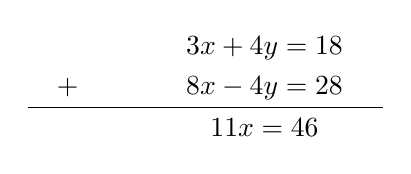
\begin{tikzpicture}
    \draw (0,0.5) node {$3x+4y=18$};
    \draw (0,0) node {$8x-4y=28$};
    \draw (-2.5, 0) node {$+$};
    \draw (-3,-0.25) -- (1.5,-0.25);
    \draw (0,-0.5) node {$11x=46$};
\end{tikzpicture}
$$
x=\frac{46}{11}, 2x-y=7 
\Longrightarrow y=2x-7
\Longrightarrow y=2(\frac{46}{11})-\frac{77}{11}=\frac{15}{11}
$$
\section{Trigonometry}

\begin{center}
If $\sin(2x) =\frac{\sqrt{3}}{2} $, and $0\degree \leq x \leq 180\degree$ what is the sum of all possible values of $x$? \\
\end{center}
Answer: $90\degree$ \\

Explanation: \\
$$
2x=60\degree,120\degree
\Longrightarrow x=30\degree,60\degree
$$

\section{Word Problem (Rates and Ratios)}
\begin{center}
A pump can fill a tank in 4 hours, while a second pump can fill the same tank in 6 hours. Both pumps work together for 1 hour, but the first pump stops. How many additional hours will it take for the second pump to fill the remaining tank?
\end{center}

Answer: 3.5 hours\\

Explanation: \\
$$
P_1(t)=\frac{1}{4}t, P_2(t)=\frac{1}{6}t
$$
$$
1=P_1(1)+P_2(1)+P_2(x)
$$
$$
1-\frac{1}{4}-\frac{1}{6}=P_2(x)
\Longrightarrow 1-\frac{3}{12}-\frac{2}{12}=P_2(x)
\Longrightarrow \frac{7}{12}=\frac{1}{6}t
\Longrightarrow \frac{7}{2}=t
$$

\section{Functions}
\begin{center}
The function $f(x)=x^3-3x^2+2x$ has the roots $r_1,r_2,r_3$, what is $r_1+r_2+r_3$?
\end{center}

Answer: $5$ \\

Explanation: \\
$$
f(x)=x^3-3x^2+2x=x(x^2-3x+2)=x(x-1)(x-2)
$$
% so it's 3

\section{Complex Numbers}
If $z=3+4i$, where $i=\sqrt{-1}$, find the magnitude of $z^2$
Answer: 25 \\
Explanation:
$$
(3+4i)^2=9+24i-16 \Longrightarrow -7+24i
$$

\section{Advanced Inequalities}

$$
|2x-5| \leq 3x + 1
$$
Answer: $-6 \leq x \leq 1$ 


\begin{align*}
    |2x-5| \leq 3x + 1 \\
    \Longrightarrow 2x-5 \leq 3x+1 \therefore -6 \leq x \\
    \Longrightarrow 2x-5 \geq -3x-1 \therefore 5x \geq 4 \therefore x \geq \frac{4}{5}
\end{align*}

\section{Unfocused Practice}

\begin{enumerate}

    \item Solve for $x$: $2^{x+1}+2^x=48$ \\

    Answer: $x=4$. 

    \begin{align*}
        2*2^x+2^x=48 \\
        2^n(2+1)=48 \\
        2^n=16 \therefore n=4
    \end{align*}

    \item If $g(x) = 3x+5$, solve for $g^{-1}(x)$ \\

    Answer: $g^{-1}(x)=\frac{x-5}{3}$

    \begin{align*}
        x=3g^{-1}(x)+5  \quad g^{-1}(x)=\frac{x-5}{3}
    \end{align*}

    \item A function satisfies $f(x+1)=2f(x)$ and $f(0)=3$. Find $f(4)$ \\

    Answer: $f(4)=48$

    From this, we can understand that each term is the next term doubled. 

    \begin{align*}
    f(x)=A2^x \\
    3=A*2^0 \\
        A=3, \therefore f(x)=3(2)^x \quad f(4)=3(2^16) \Longrightarrow f(4)=3(16) 
        \Longrightarrow f(4)=48
    \end{align*}

    \item A triangle has sides 5, 12, $x$. If $x$ is an integer, find all possible values of $x$. \\
        
    Answer: $7 \leq x \leq 17$ 

    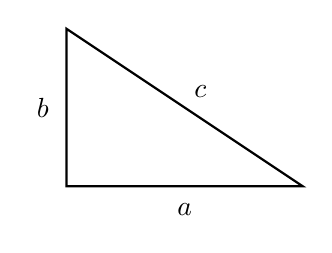
\begin{tikzpicture}
        \draw [thick] (0,0) -- (3,0) -- (0,2) -- cycle;
        \draw (1.5,-0.3) node {$a$};
        \draw (-0.3,1) node {$b$};
        \draw (1.7,1.2) node {$c$};
    \end{tikzpicture}

    No side can be greater than the other two or less than the difference.

    \begin{align*}
        c<a+b 
        \quad c>|a-b|
        \Longrightarrow x < 5+12 \quad x > |12 - 5| \\
        \therefore 7 < x < 17
    \end{align*}

    \item Find the area ($a$) of a right triangle with hypotenuse length of 13 and one leg length of 5. \\

    Answer: $a=30$ \\

    Since the triangle is right, we can use $a^2+b^2=c^2$. 

    \begin{align*}
        5^2+b^2=13^2 \\
        b=\sqrt{13^2-5^2} 
        \Longrightarrow b=12
    \end{align*}
    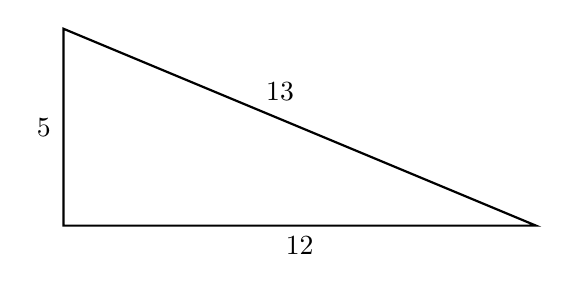
\begin{tikzpicture}[scale=0.5]
        \draw [thick] (0,0) -- (12,0) -- (0,5) -- cycle;
        \draw (6,-0.5) node {$12$};
        \draw (-0.5,2.5) node {$5$};
        \draw (5.5,3.4) node {$13$};
    \end{tikzpicture} \\
    Since $a=\frac{1}{2}bh$, we can use $a=\frac{1}{2}(5)(12)$ and get $a=30$.

    \item A circle is centered at $(4, -3)$ and is tangent to the line $y=2$. Find its radius, $r$. \\
    Answer: $r=5$ \\

    \begin{tikzpicture}[domain=-1:6]
        % draw a circle
        \draw[very thin,color=gray] (-0.1,-5.1) grid (5.1,2.1);
        \draw[fill=black] (4,-3) circle [radius=0.1];
        \draw plot (\x,2) node[above] {$y=2$};
    \end{tikzpicture}

\end{enumerate}
\end{document}
